In this section, we take a close look at the proposed structure and capabilities of the framework's API.
The final implementation will however deviate with a high probability.

\subsection{Proposed Functionality}

The framework shall have two primary capabilities: first, it should enable fast and easy access to the 3d space calculated from the marker.
Second, given a model to display, it should be capable of returning a rendering of the object within the scene.

Generally, the framework shall work like in the following.
Upon import of the framework into the project, the program passes the image to the framework.
This shall be possible to do in two ways: one, let OpenCV read directly from the camera, or two, give the framework the frames from the program manually.
This allows the possibility of using other video or picture streams with the framework\footnote{For example, rendering an object into a video.}.

Now the magic happens; OpenCV calculates the 3d space.
Before passing it on to the framework, the program can read the 3d space.
This direct access to the resulting coordinate space allows a more down-to-earth programming should it be required.
If the program is only interested in the final rendered frame, given a model, the framework then renders the object into the scene and returns the frame to the program.

\begin{figure}
	\centering
	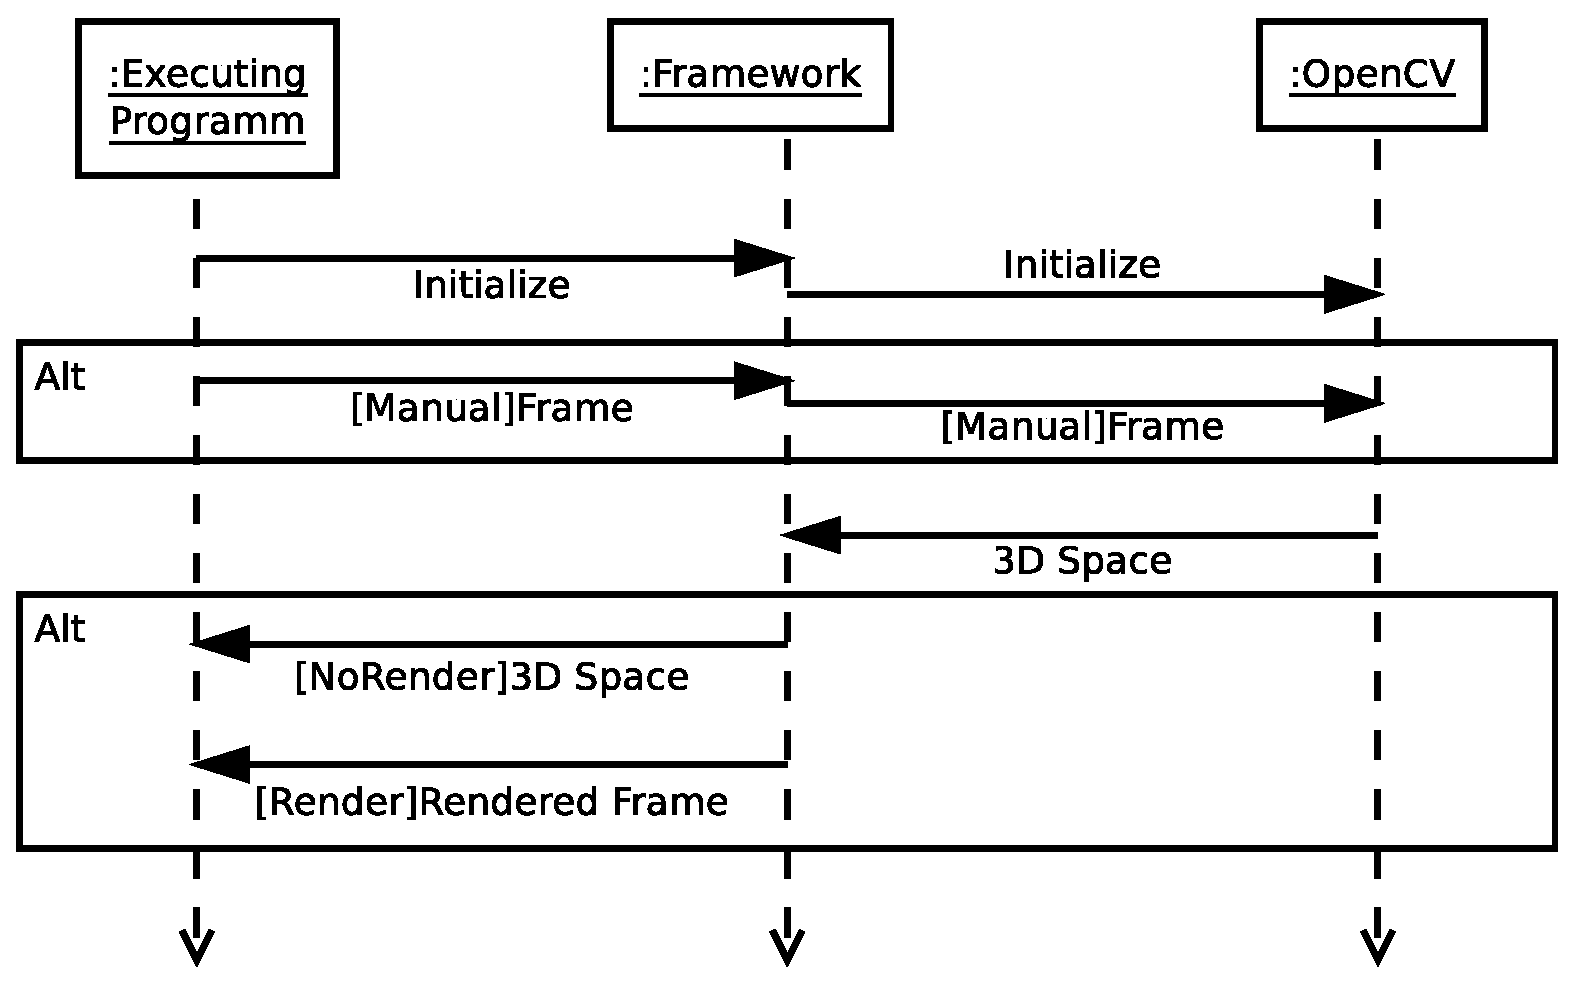
\includegraphics[width=12cm]{images/sequence_access.eps}
	\caption[Access Sequence.]{The proposed sequence of the workflow with the framework, using OpenCV.}
	\label{fig:sequence_access}
\end{figure}

Figure \ref{fig:sequence_access} shows the proposed outside view of the framework, and where data can be input or read.
As proposed, the framework should offer a wide variety of uses, without being overly complex.
Another important aspect we want to make possible is the possibility of changing all the more important parameters during runtime, such as switching the model or adding a new marker.
This should allow a much smoother usage of the framework and any derived apps as a result.

\subsection{Application Interface}

The following represents the suggested interface for the framework.
With the listed methods, all functionality that the framework offers can be accessed.

TODO: Place javadoc here.

\subsection{Usage}

\begin{figure}
	\centering
	
\includegraphics[width=4cm]{images/marker_example.png}
	\caption[Example Marker.]{An example of a marker. This image is either printed or displayed by some other means in the real world to allow a system to use it as a reference to base a virtual overlay off of it.}
	\label{fig:marker_example}
\end{figure}

To enable the framework to detect a 3d coordinate system from a video feed, a marker will be required.
A marker is a visually significant pattern that the system can detect within an image and be used to calculate spatial coordinates. Figure \ref{fig:marker_example} shows an example for such a marker.

Depending on the capabilities of the finished framework, it could be possible to track multiple markers in a single instance.
This would allow multiple objects to be rendered simultaneously, increasing the use cases for the framework.

To enable the functionality, the recorded or live video stream must have a pre-defined marker somewhere in it.
This can be a screen showing the marker, a printed marker, or any other way of displaying a marker in a scene.
Depending on the capabilities of OpenCV, the framework will then detect its relative 3d position.
With the detected space, the framework can now render objects into the scene with the correct rotation, scaling, and perspective.

